\chapter{AR Library}
\label{chp:AR Library}

Beside the before mentioned potential power of the library as a reasons in favor of choosing \textit{Awe.js} it is worth to observe this library in more details to be able to estimate whether it is actually a good choice in terms of technical facilities.

\section{Awe.js}

As \textit{Awe,js} provides examples of marker detection as well as of a stereoscopic effect it can be assumed, that those two can be combined. Looking at the code it reveals that \textit{Aws.js} not only sits on top of \textit{Three.js} but also on a bunch of other libraries combined to achieve certain tasks. 
 
In the old GitHub repository - the \textit{buildAR.com} version - the \textit{Awe.js} team titled the page with \textit{The jQuery for the Augmented Web}. I interpret this as they wanted to say, that they provide one single API that is more user friendly many combining complicated functions of different APIs such as WebRTC, WebGL or WebVR. They actually provide such an API that is described in the \textit{README.md}\footnote{Online on GitHub at \url{https://github.com/awe-media/awe.js/blob/deprecated/README.md}.} of the deprecated version - the one used for this project. According to the newest \textit{README.md}\footnote{Online on GitHub at \url{https://github.com/awe-media/awe.js/blob/master/README.md}} on GitHub "the awe.js API sits on top of THREE.js and makes it easy for you to manage scenes, media objects, interactivity, sensors, device types and more." 

The fact that \textit{Awe.js} even sits on top of \textit{Three.js} that handles itself some of those APIs shows that \textit{Awe.js} is high level in the sense of being far away from the actual task being done. This will make it hard to adapt some functionalities, when a library at a lower level does not perform as desired.

As long as \textit{Awe.js} serves the purpose helping to achieve the projects goal there is no reason not to use it. Important to know is that the both \textit{README.md} files a brief manual to the \textit{Awe.js} API. 


\section{Base Code}
\label{sec:baseCode}

There are several examples from the \textit{Awe.js} ZIP-archive that could serve as the base code. However, as mentioned in the Chapter \ref{chp:introduction} the project will use the marker based approach. Therefore the example showing the use of a marker serves this purpose best and is copied to the \textit{Applications/Chapter3} folder. 
Adapting and simplifying this, it becomes the \textit{baseCode.html} file.
All needed files are copied into the \textit{third-party} folder. 

For the following steps it is helpful to have the marker printed out. The size does not matter. The size 6cm x 6cm works grate for me. Folding the paper to create a doubled layer paper stabilizes the marker and eases the use of it. It might be even printed on cardboard. 

To minimise confusion, the cube with the fixed position is removed. The only object that is left is the other cube that will show up, when the marker \textit{64.png} - shown in figure \ref{fig:marker} - is detected.
Knowing the problem of loading textures for launching \textit{baseCode.html} locally the texture is removed. As this results in a cube without visible inner edges according to what was learned in the previous section it has to do with the material or the light. Comparing with the other examples it shows that the additional ambient light does not work out in the desired way and therefore it is removed too. This results in a quite clean demonstration of the basic function of the marker detection. When running {baseCode.html} it places a white cube on the place where the marker is presented like shown in figure \ref{fig:cube on marker}.

\begin{figure}
	\begin{subfigure}[t]{0.45\textwidth}
		\centering
		
\includegraphics[height = 3.5cm]{Document/Figures/chapter3/64}
		\caption{}
        \label{fig:marker}
	\end{subfigure}
	\hfill
	\begin{subfigure}[t]{0.45\textwidth}
		\centering
		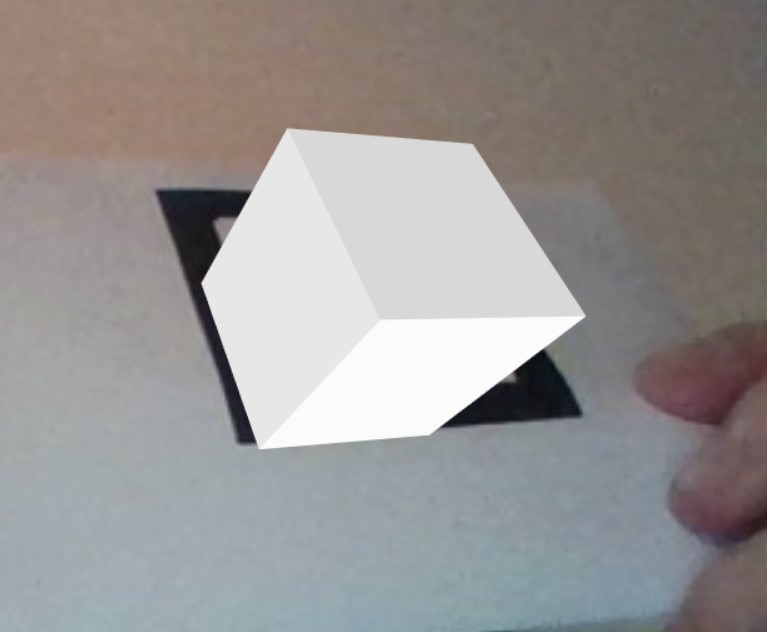
\includegraphics[height = 3.5cm]{Document/Figures/chapter3/ScreenshotMarkerDetectedWhiteCube.jpg}
		\caption{}
        \label{fig:cube on marker}
	\end{subfigure}
	\caption[Marker and Cube]
			{(a) used marker 64.png
			 (b) cube placed on recognised marker}
\end{figure}

Abel to run {baseCode.html} locally without problems there are now some restrictions showed for the server use. Because \textit{Awe.js} uses \textit{deviceorientation event}, \textit{devicemotion event} amd \textit{getUserMedia()} the browser will block, when a non secured origin is assumed. \textit{http://localhost} and HTTPS is treated as secure and will work. For more details are provided at \url{https://goo.gl/rStTGz}.

Black box testing shows that the marker detection works best when the camera is facing the surface where the marker is placed on perpendicular. For shallow angles the detection does not work. The angles between are able do be detected however it reveals that the placement is not really accurate. 
Lets define the z-axis as the line perpendicular to the marker and towards the camera. When the marker is rotated around the z-axis the object rotates accordingly. Doing a rotation of the marker around the corresponding x- or y-axis the object will rotate too however around a different point which leads to a displacement of the otherwise centered object. It looks like the center of rotation for the object is set at ts center - what is bad if it should stand on the marker - and that the object itself is not really on the marker but somehow a bit too close to the camera in respect to the marker. Trying to use different sizes for  the marker leads to the same observation.

To handle this problem it can either be solved in a programmatic way or be bypassed with some restrictions to use. 

Finding the actual place where the faulty behaviour is generated could be very cumbersome due to the structure of \textit{Awe.js}. A first step could be to use the hidden debug mode that seems to allow the debugging of the marker detection. To activate it the variable \textit{DEBUG} has to be set to \textit{true} before the loading of the dependencies and the \textit{window.awe.init(...)} function. The calculation are done in the file \textit{awe.marker\_ar.js} that is located in \textit{third-party} folder. Examining this file I found out that the manipulation is done to the property \textit{mesh} - and applied to its matrix - that can also be accessed via the \textit{Awe.js} API. As I prefer to leave the third-party code unchanged and to ease a possible reproduction of this work I choose to take the bypass solution.

The original idea to set a marker on a table and setting a chess figure on it will not work due to the angle that will be created when looked from the side on it. As it is not practically to tell the user to watch from top down onto the marker it is easier to place the marker differently. Therefore the bypass for the problem is thinking of the marker as being on the wall or it is hold like a book the optimal angle can be provided to let \textit{Awe.js} work as expected. There are enough application ideas that can use exactly this configuration - e.g. a book with interchangeable content. As a side effect this will result in a more natural user experience as user can look straight away and does not have to look down. When moving the marker the user simply has to follow it. This may sounds like a big restriction. However enabling the marker to be more than just a location for an digital object and let it equally be a controller. As the rotation around the z-axis works it could as sort of steering wheel. Even the use of different markers can be considered thinking of a wall putting different object to.

It is also recommended to have a good lightning conditions. If the marker that has to be detected is not sufficiently lighted the detection starts flickering.

\section{Building Enhanced Scene }
\label{sec:enhancedScene}

Taking \textit{baseCode.html} as template \textit{enhancedScene.html} is created. Adding the \textit{dat.GUI} - like in the previous chapter in section \ref{sec:Manipulating Objects} - to ease later manipulation of the Scene. 

The \textit{Awe.js} API is indeed quite easy to understand. There are \textit{pois} representing places and \textit{projections} are the actual objects. A \textit{projection} can the be added to a \textit{poi}. A \textit{poi} can also be added to another \textit{poi}. It can be helpful when placing object to put them first on a fixed position first to see how they will be placed. The coordinate system is as usual with x as the horizontal axis, y the vertical axis and z the axis perpendicular to the screen. 
For some reason the \textit{poi} that is attached to the marker will be rotated 180 degrees around the y-axis and also 180 degrees around the z-axis. A simple workaround is to attach a second poi to the poi that is attached to the marker and rotated this one accordingly. The poi directly attached to the marker get its rotation from the marker and can not be manipulated manually.
The result of this application is shown in figure \ref{fig:enhancedScene}. 

\begin{figure}[h]
    \centering
    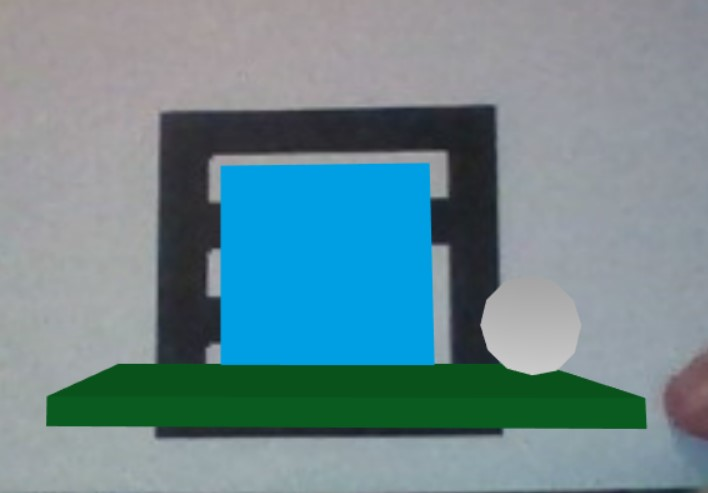
\includegraphics[height=4cm]{Document/Figures/chapter3/ScreenshotMarkerDetectedEnhancedScene.jpg}
    \caption[Screenshot enhanced scene on marker]{Screenshot enhanced scene attached to detected marker when  running \mbox{\textit{enhancedScene.html}}}
    \label{fig:enhancedScene}
\end{figure}


\section{Marker as Controller}
\label{sec:markerController}

The previous HTML file was copied and renamed to \textit{markerController.html}. The aim is to control the ball by rotating the marker. As found out in section \ref{sec:baseCode} the properties of the detected marker are applied to the matrix of the mes from the poi. It can be accessed via \mbox{\textit{awe.pois.view(id).get\_mesh().matrix}}.

To be able to have an animation beside the \textit{Awe.js} API a independent animation function is added. 
Using the fact, that \textit{Three.js} is on board it is easy to get the angle around z by calling the integrated functions. As \textit{Three.js} has to be loaded first its not available at the top. Using it somewhere inside the \textit{window.awe.init} will be fine as it waits until the window is loaded and therefore \textit{Three.js} too. In the resulting application the ball can be moved from left to right and back bei steering with the marker.

\section{Evaluation}

Shows possibility of marker
crud


